\documentclass[11pt]{article}
% Adapted from an original template by Hlyni Arnórssyni,
% Reykjavik University, Iceland

% pgfplots loads xcolor first, so pass the table option early to avoid an option clash.
\PassOptionsToPackage{table}{xcolor}

% ------------------------------ PAGE SETTINGS ------------------------------
\usepackage{geometry}

\geometry{
    paper=a4paper,
    top=2.5cm,
    bottom=2.5cm,
    left=2.5cm,
    right=2.4cm,
    headheight=0.75cm,
    footskip=1.5cm,
    headsep=0.75cm
}

% ------------------------------ BASIC PACKAGES ------------------------------
\usepackage{blindtext}

% Character encoding
\usepackage[T1]{fontenc}
\usepackage[utf8]{inputenc}

% Mathematics
\usepackage{amsmath, amsfonts, amsthm, amssymb}
\usepackage{braket, nicefrac}

% SI units
\usepackage{siunitx}

% Lists / columns
\usepackage{enumitem, multicol}

% ------------------------------ FIGURES ------------------------------
\usepackage{graphicx}
\usepackage{float}
\usepackage{keystroke}
\usepackage{pgfplots}
\usepgfplotslibrary{units}
\pgfplotsset{compat=1.16}

% Search these locations automatically for figures
\graphicspath{{fig/}{graphics/}{Graphics/}{./}}

% ------------------------------ TABLES ------------------------------
\usepackage{tabularx}
\usepackage{array}
\usepackage[table]{xcolor}

% ------------------------------ TYPOGRAPHY ------------------------------
\usepackage{caption}
\usepackage{titlesec}
\usepackage{microtype}
\usepackage{csquotes}

% ------------------------------ COLORS ------------------------------
\definecolor{GWBlue}{HTML}{1E4E79}

% ------------------------------ SECTION STYLING ------------------------------
\titleformat{\section}
  {\Large\bfseries\color{GWBlue}}
  {\thesection.}
  {0.40em}
  {}

\titlespacing*{\section}
  {0pt}
  {0.70em}
  {0.28em}

% ------------------------------ CAPTION STYLING ------------------------------
\captionsetup{
    font=small,
    labelfont=bf,
    textfont=it,
    labelsep=period,
    skip=4pt
}

% ------------------------------ PARAGRAPH SPACING ------------------------------
\setlength{\parindent}{0pt}
\setlength{\parskip}{0.30em}

% ------------------------------ BIBLIOGRAPHY ------------------------------
\usepackage[
    backend=biber,
    style=authoryear,
    sorting=none,
    giveninits=true,
    maxbibnames=99,
    dashed=false
]{biblatex}

\addbibresource{references.bib}

\DeclareNameAlias{sortname}{family-given}
\DeclareNameAlias{default}{family-given}
\DeclareFieldFormat[article]{title}{#1}
\DeclareFieldFormat[misc]{title}{#1}
\renewbibmacro{in:}{}

\AtEveryBibitem{%
    \clearfield{doi}%
    \clearfield{urldate}%
}

\AtBeginBibliography{\small}
\setlength{\bibitemsep}{0.35em}

% ------------------------------ HYPERLINKS ------------------------------
\usepackage{hyperref}

\hypersetup{
    colorlinks=true,
    linkcolor=GWBlue,
    citecolor=GWBlue,
    urlcolor=GWBlue
}
\usetikzlibrary{arrows.meta,positioning,fit,backgrounds}
\newcolumntype{C}[1]{>{\centering\arraybackslash}p{#1}}

\begin{document}

\begin{center}

\includegraphics[width=0.28\textwidth]{gwu_logo.pdf}\par\vspace{4pt}
{\Large\bfseries Where Do Neural Networks Fail?\par}
{\large\bfseries Post-Training Analysis and Novelty Detection Using\\ Neural Network Self-Organizing Maps (NNSOM)\par}
\vspace{6pt}
{\normalsize Capstone Group 5: Fyrooz Anika Khan, Nazish Atta\par}
{\small DATS 6501 Capstone, Fall 2026, The George Washington University. Supervised by Dr.\ Amir Jafari.\par}
\end{center}

\begin{abstract}
\noindent We ask where a convolutional network (CNN) fails and whether a self-organizing map (SOM) trained on its internal features can help. A LeNet-5 reaches 99.18\% test accuracy on MNIST. On a 15$\times$15 SOM its few mistakes gather in 11 cells that hold 11.1 times their fair share, but the CNN's own confidence finds mistakes better than the map does (AUROC 0.981 against 0.685).
As a novelty detector, the SOM's quantization error separates SVHN images from MNIST well (AUROC 0.981), yet energy (0.9998) and max-softmax (0.9985) do better. What the SOM adds is a picture of \emph{where}: the SVHN images land on only 28 of the 225 cells.
In a harder test, where the networks are trained on 6 digits and the other 4 are new, the SOM still detects the new digits (mean AUROC 0.912 over five class splits), but plain nearest-neighbor distance does better in every split (0.966), and the comparison with max-softmax (0.944) is inconclusive.
Used to guide retraining, SOM-chosen hard images with altered copies cut the mistakes in the error cells from 11.4\% to 7.8\% over five seeds, without raising the error elsewhere. Choosing the images the CNN is least sure about worked about as well, and letting the hard images in slowly (curriculum learning) made the CNN worse.
New SOMs trained on the retrained CNNs have smaller weak regions but not purer cells, and the SOM still detects SVHN after retraining.
Our main contribution is to show that, as a guide for retraining, the SOM does as well as the CNN's own confidence, and that unlike that confidence it also shows where the errors cluster and why: in a few cells where two digit classes overlap.
Every result is compared with a control or a chance level, and unmeasured items are marked.
\par\smallskip
\noindent\textbf{Keywords:} self-organizing map, post-training analysis, error analysis, novelty detection, MNIST.
\end{abstract}

\section{Introduction}

A neural network can be right 99\% of the time and still make mistakes that follow a pattern. Our starting model is a LeNet-5 network \parencite{lecun1998gradient}. It reads handwritten digits from the MNIST dataset and gets 99.18\% of the test images right (86 mistakes in 10,500 images).
The question we ask is: where do these few mistakes come from?

Well-known tools such as saliency maps \parencite{simonyan2014saliency}, LIME \parencite{ribeiro2016lime} and SHAP \parencite{lundberg2017shap} explain one prediction at a time.
They do not show where, inside the network, the mistakes gather.

We use a Self-Organizing Map (SOM) \parencite{kohonen1990som} to get this wider view. A SOM places data on a flat grid so that similar items end up in nearby cells. We use the NNSOM library \parencite{jafari_nnsom}.
The plan is to train the CNN first, then record the 84 numbers it computes for each image just before it answers (the \emph{embedding}), and then train a SOM on these embeddings. We ask three questions:
(i)~where on the map do the CNN's mistakes gather; (ii)~can the map spot inputs that are unlike the training data; and (iii)~can the map choose better samples for retraining than random choice?
Because the SOM is trained on the CNN's own embeddings, we also check whether it tells us more than simple methods do, and we compare the plain CNN with a SOM-assisted CNN from start to finish (Figure~\ref{fig:endtoend}).

\textbf{Contributions.}
(1)~A repeatable CNN and SOM pipeline for MNIST.
(2)~Evidence that the CNN's mistakes gather in a small set of cells of a 15$\times$15 map, where digits overlap. This is tested against chance.
(3)~A comparison with simple baselines. It shows that this pattern is not special to the SOM, and that the CNN's own confidence is a much stronger signal for finding mistakes.
(4)~Tests of the SOM as a novelty detector (MNIST against SVHN, compared with energy, max-softmax, Mahalanobis, nearest-neighbor, Isolation Forest, One-Class SVM and autoencoder scores) and as a guide for retraining (against random and least-confident choices, five seeds each). The SOM did not beat the simple baselines at either job. Its value is that it shows where the errors and the novel inputs sit.

\section{Related Work}

Our work touches four areas of research. For each one we say what it does and how our work is different.

\textbf{CNNs as a source of features.} LeNet-5 \parencite{lecun1998gradient} showed that convolutional networks learn useful features for handwritten digits. We do not propose a new classifier.
We train LeNet-5 with the Adam optimizer \parencite{kingma2015adam} and then keep it fixed, so we can study how it organizes its features and where it fails.

\textbf{Explaining single predictions.} Saliency maps \parencite{simonyan2014saliency} show which pixels change a class score the most. LIME \parencite{ribeiro2016lime} fits a simple model around one prediction.
SHAP \parencite{lundberg2017shap} gives each input feature a share of the credit. All three answer the question ``why this prediction?''. We ask a different question, ``where in the network's features do mistakes gather?'', so our work adds to theirs.

\textbf{Self-Organizing Maps.} Kohonen's SOM \parencite{kohonen1990som} puts data on a flat grid so that nearby cells hold similar data. Vesanto and Alhoniemi \parencite{vesanto2000clustering} showed how to group the cells of a trained SOM and measure the result.
NNSOM \parencite{jafari_nnsom} provides the training code and the quality measures we use. SOM-VAE \parencite{fortuin2019somvae} and DESOM \parencite{forest2021desom} train the features and the map together.
We do the opposite on purpose. We keep the CNN fixed, so any signal from the SOM can be judged on its own.

\textbf{Finding systematic errors.} Domino \parencite{eyuboglu2022domino} looks for groups of data where a model does badly and describes them in words. The Spotlight \parencite{deon2022spotlight} searches the feature space for a region where the model's loss is high.
These are closest to our error analysis. We differ in two ways. We use a map that keeps neighbors close, which gives one fixed picture that a person can read. And we test every claim against chance and against simple baselines.

\textbf{Novelty and out-of-distribution detection.} Hendrycks and Gimpel \parencite{hendrycks2017baseline} proposed the maximum softmax probability (the network's top probability) as a simple baseline for finding mistakes and unfamiliar inputs.
ODIN \parencite{liang2018odin} improves it with a temperature setting and small changes to the input. Lee et al.\ \parencite{lee2018mahalanobis} measure distance to each class in feature space, and Liu et al.\ \parencite{liu2020energy} use an energy score.
Deep SVDD \parencite{ruff2018deep} learns a compact description of normal data, and Sun et al.\ \parencite{sun2022knn} show that the distance to the nearest training features works well. The survey by Yang et al.\ \parencite{yang2024generalized} puts these methods side by side.
We do not claim that a SOM beats them. We test whether the SOM's own measures give a useful novelty signal, while also giving a picture of where mistakes sit.

\textbf{Other novelty detectors we compare with.} Isolation Forest \parencite{liu2008isolation} isolates unusual points by random splits, and the One-Class SVM \parencite{scholkopf2001support} learns a boundary around normal data. An autoencoder flags inputs it rebuilds badly \parencite{sakurada2014autoencoder}.
We run all three on the CNN's embeddings. Nalisnick et al.\ \parencite{nalisnick2019deep} showed that models of normal data can rate unfamiliar images as \emph{more} typical, which is the pattern we see for two of these detectors on SVHN (Section~\ref{sec:p3results}).

\textbf{How our work differs.} Earlier work either explains single predictions, trains maps together with the model, or detects novelty without showing where the failures sit. We use one SOM on fixed features for all three jobs: finding mistakes, detecting novelty, and guiding retraining.
We test each claim against chance and against simple baselines. This already changed one conclusion: on MNIST the pattern of mistakes is real, but a plain k-means grouping and the CNN's own confidence do as well or better at finding them (Table~\ref{tab:error-pattern-baselines}).

\section{Method}
\label{sec:method}

\subsection{Data and model}

MNIST is split once into 49,000 training, 10,500 validation and 10,500 test images. The split keeps the same share of each digit in every part, and it uses a fixed random seed so it can be repeated.
We train a LeNet-5 with Adam \parencite{kingma2015adam} and keep the version with the best validation accuracy. For every image we then record the 84 numbers from the network's second-to-last layer (called fc2). These numbers are the embedding.
We rescale them to the range $-1$ to $1$, using the training data only (Figure~\ref{fig:pipeline}).

\begin{figure}[H]
\centering
% Diagrams are drawn in draw.io: each has an editable .drawio source, a .drawio.svg export and the PDF used here, all in fig/diagrams/.
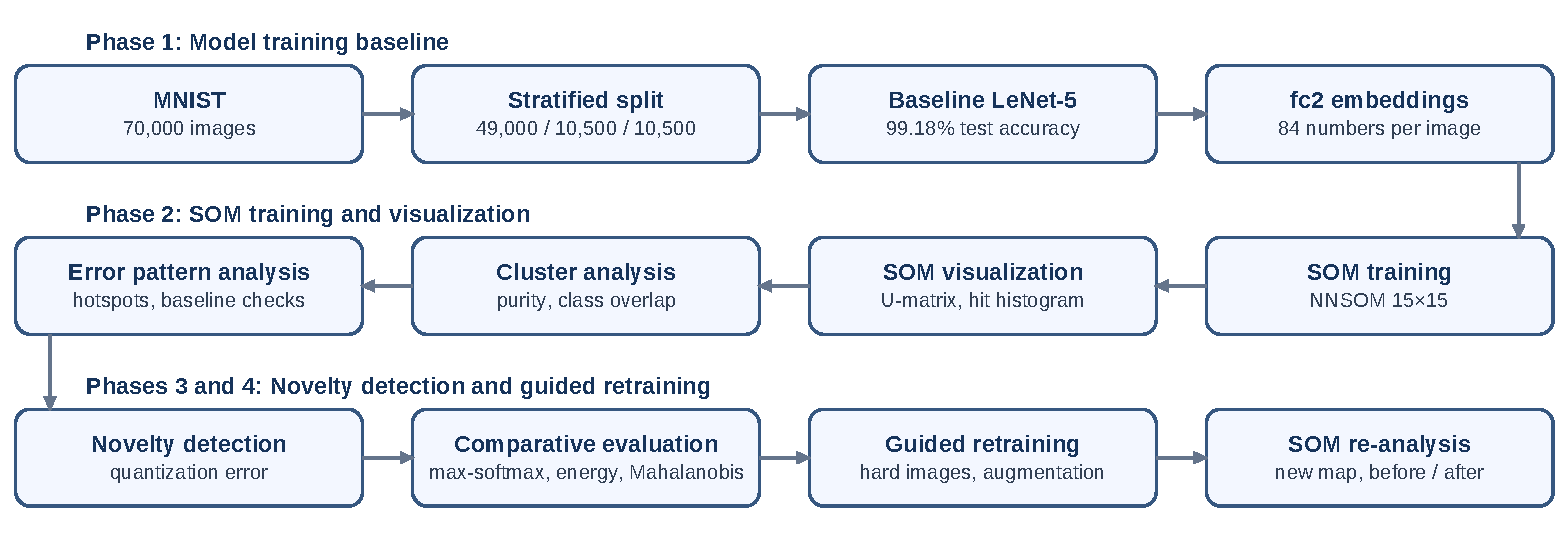
\includegraphics[width=\linewidth]{diagrams/project_pipeline.pdf}
\caption{The project pipeline, from the baseline CNN (Phase 1) and the SOM (Phase 2) to novelty detection (Phase 3) and guided retraining with a new SOM (Phase 4).}
\label{fig:pipeline}
\end{figure}

\subsection{Self-Organizing Map}

A SOM is a competitive network: a layer of neurons, each with a weight vector of the same length as the input, arranged on a grid \parencite{kohonen1990som,hagan2014nnd_ch16}. For each input, the neurons compete, and the one whose weights are closest wins. The winner and the neurons near it on the grid then move their weights toward the input. Because neighbours learn together, neighbouring cells end up holding similar inputs, so the grid becomes a flat picture of the data. Figure~\ref{fig:som_explained} shows these steps for our project.

\begin{figure}[H]
\centering
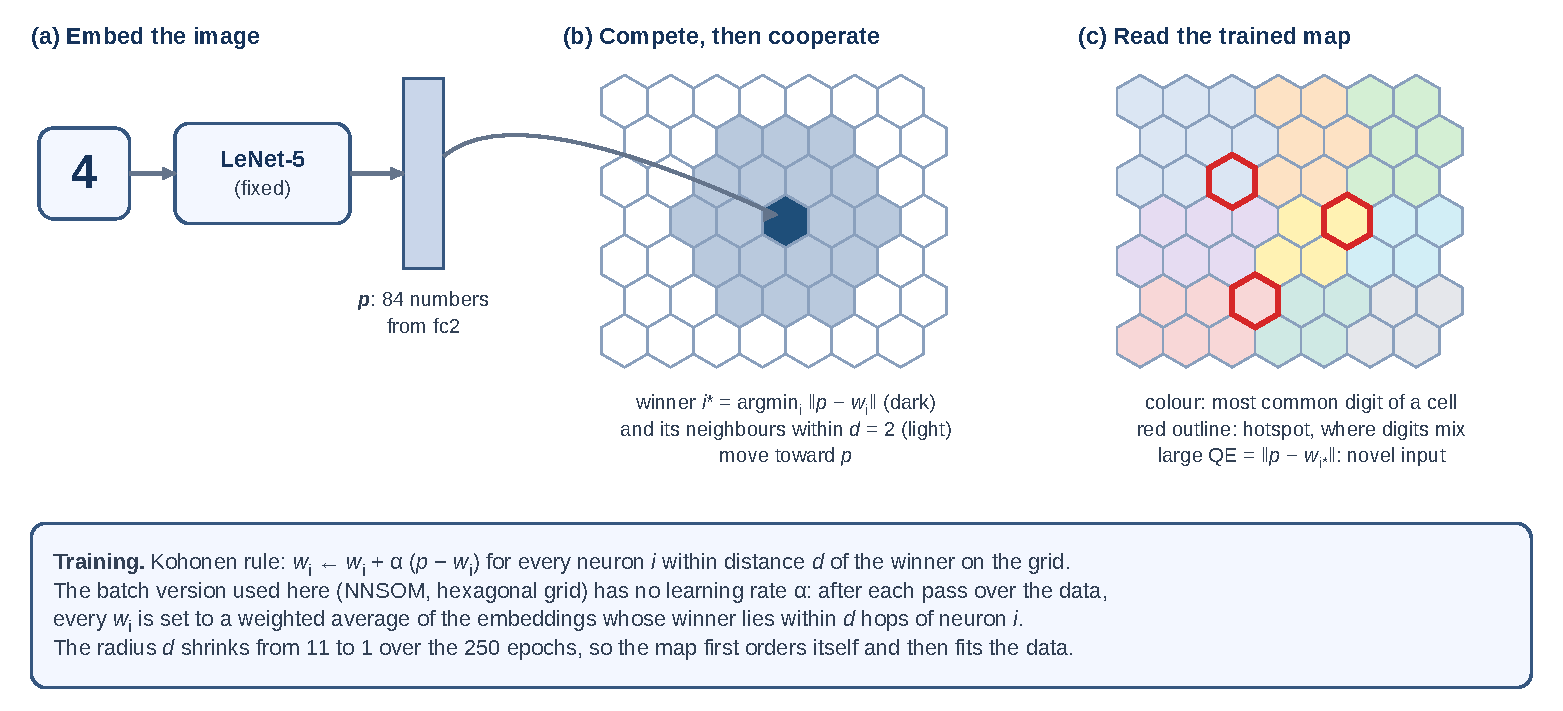
\includegraphics[width=\linewidth]{diagrams/som_explained.pdf}
\caption{How the self-organizing map works in this project, following the competitive-network chapter of \textcite{hagan2014nnd_ch16} and its batch version \parencite{hagan2014nnd_ch26}. (a)~Each image is turned into an 84-number embedding by the fixed CNN. (b)~The neuron whose weight vector is closest wins, and the winner and its grid neighbours move toward the embedding, so neighbouring cells end up holding similar images. (c)~After training, each cell is labelled by its images: their most common digit, how mixed the digits are, and how often the CNN is wrong there (hotspots). An image far from its best cell (large quantization error, QE) is unlike the training data. The grids are schematic; the real map has 15$\times$15 hexagonal cells.}
\label{fig:som_explained}
\end{figure}

We train a 15$\times$15 map (225 cells) on the 49,000 training embeddings with the batch rule of NNSOM \parencite{jafari_nnsom,hagan2014nnd_ch26}. Each image is assigned to the cell whose weights are closest to it, called its best-matching neuron (BMU).
We judge the map with two numbers. The quantization error (QE) is the average distance between an image and its cell. The topological error (TE1) is the share of images whose two closest cells are not neighbors on the grid.

We tried three grid sizes (10$\times$10, 15$\times$15 and 20$\times$20) under the same conditions: the same data, three starting neighborhood sizes, ten maps per grid, and validation data only.
Larger grids fit the data more closely (QE 1.21, 1.06 and 0.98) and have slightly purer cells (97.6\%, 98.2\% and 98.4\%), but they also have a higher topological error (TE1 4.8\%, 6.6\% and 7.7\%).
The grids are not clearly different at predicting the CNN's mistakes: the AUROC difference between 20$\times$20 and 15$\times$15 is $+0.001$ (95\% range $-0.100$ to $+0.089$), so the comparison is inconclusive.
Since no grid is clearly better, we use the 15$\times$15 map for the main analysis. It has good purity and a lower topological error than the 20$\times$20 map.
We repeat the error analysis on the other two grids to check that the conclusions do not depend on this choice.
As a further check on the settings, we tuned the starting neighbourhood size and the number of epochs of each grid with Optuna's TPE sampler \parencite{akiba2019optuna}: 20 trials per grid, scored on validation QE and TE1 only, followed by five new training seeds for the best setting. For the 15$\times$15 map the tuned setting was not clearly better than ours (QE $+0.005$, 95\% interval $-0.003$ to $+0.013$; TE1 $-0.14$ points, $-0.81$ to $+0.53$), so the map used in this report stays the same. Tuning did find a better 10$\times$10 setting; that grid is used only for the robustness check.

\subsection{Finding where mistakes gather}

For each cell we compute its \emph{purity} (the share of its images that belong to its most common digit) and the \emph{entropy} of its digit mix (how mixed the digits are). We compare the overall purity with a chance level. To get the chance level,
we shuffle the digit labels 1,000 times and measure the purity again.

To find hotspots, we rank the cells by the lower end of the 95\% Wilson interval \parencite{wilson1927probable} of their error rate. This keeps small cells from ranking high by luck.
The top $\max(5,\,5\%\text{ of the cells})$ are the hotspots. We pick hotspots using a random half of the validation images and measure them on the other half, using the \emph{concentration ratio}:
\[
\text{ratio}=\frac{\text{share of the mistakes that fall in hotspots}}{\text{share of the images that fall in hotspots}}.
\]
A ratio of 1 means the mistakes are spread evenly. We repeat this over 200 random half-splits and report the median. Chance is estimated by repeating everything 200 times with the mistake labels shuffled.
We also compute the Spearman correlation between a cell's error rate and its purity and entropy, to see whether mistakes sit where digits overlap.

\subsection{Comparison with simple baselines}

We repeat the analysis with three simple methods: (a)~k-means with 225 clusters (the same number as SOM cells); (b)~the impurity of the 15 nearest training embeddings; and
(c)~the network's maximum softmax probability \parencite{hendrycks2017baseline}, meaning how sure the network is of its answer.
Each score is judged on the same validation images by the area under the ROC curve (AUROC), which says how well the score separates mistakes from correct answers (1 is perfect, 0.5 is chance). We give bootstrap confidence intervals.
None of these methods depends on the dataset, so they can also be used on Fashion-MNIST.

\subsection{Phase 3: Novelty detection}

Here the SOM and the CNN stay fixed, and we ask whether an image that is unlike MNIST gets a score that marks it as new. The normal (in-distribution) images are the 10,500 MNIST validation images. The novel (out-of-distribution) images are the 26,032 images of the official SVHN test set, which show house numbers from street photos.
We use two scores from the SOM. The first is the quantization error (QE): the distance between the image's embedding and its best cell, so a larger value means the image fits the map less well. The second is the U-matrix score: the distance between the image's cell and its neighbors on the grid.
We compare them with seven other scores computed on the same embeddings or logits: the maximum softmax probability, the energy score \parencite{liu2020energy}, the Mahalanobis distance \parencite{lee2018mahalanobis}, the distance to the nearest training embeddings \parencite{sun2022knn}, Isolation Forest, One-Class SVM and an autoencoder.
A random score serves as the null.

We report the AUROC, which tells how well a score ranks novel images above normal ones (1 is perfect, 0.5 is chance), the AUPR (novel images are the positive class), and the false-positive rate when 95\% of the novel images are caught (FPR at 95\% TPR). Intervals are bootstrap intervals from 2,000 resamples.
For the QE detector the alarm threshold is the 95th percentile of the QE of the training images (1.569), fixed before looking at SVHN. We did not change any setting after seeing the SVHN results.
\textbf{Near novelty: held-out digits.} SVHN is very unlike MNIST, and its embeddings are much shorter, so it is an easy test. For a harder one we follow the open-set setup for MNIST \parencite{neal2018open}: in each of five class splits, 6 digits are known and 4 are unknown, drawn at random once and fixed before any run. For each split we train a new LeNet-5 (Phase 1 recipe) and a new 15$\times$15 SOM (Phase 2 recipe) on the training images of the known digits only. The normal images are the validation images of the known digits; the novel images are the validation images of the unknown digits. We compare QE with max-softmax, energy, Mahalanobis and nearest-neighbor distance. Max-softmax is the strong baseline in this setting \parencite{vaze2022openset}. The protocol, the splits and the four statements were written down before the run: (H1) the SOM detects the held-out digits; (H2, the main one) it is better than max-softmax; (H3) it is no more than 0.01 AUROC worse than max-softmax, energy or Mahalanobis; (H4) it is better than nearest-neighbor distance. Each is tested with a 95\% t-interval over the five splits and can be shown, shown to be the opposite, or inconclusive.
Fashion-MNIST is left for the next datasets and is not part of these results.

\subsection{Phase 4: Guided retraining}

Here we use what the map shows to retrain the CNN, and then look at the map again (Figure~\ref{fig:loop}). The retraining recipe is the Phase 1 recipe (Adam, 20 epochs), repeated for 5 seeds with the same seeds for every method, and it uses the training images only.
A training image is called \emph{hard} if its cell is one of the 11 error hotspots, or its cell has a purity below 0.95, or it lies unusually far from its cell (above the 95th percentile). This gives a pool of 4,217 of the 49,000 training images (8.6\%).
We retrain in two ways. In \emph{curriculum learning} the CNN starts with the easy images plus 10\% of the hard pool, and more hard images are added every 5 epochs. In \emph{targeted augmentation} we add three slightly changed copies (small turns, shifts of at most 1 pixel, zoom and shear) of every hard image to the training data.
Each way has controls that use the same number of images: random images, the images with the lowest maximum softmax probability, and a gradual version of the augmentation. The success criteria were written down before the test images were used. The paired differences between methods have bootstrap intervals over the test images.
The test images were used once.

\begin{figure}[H]
\centering
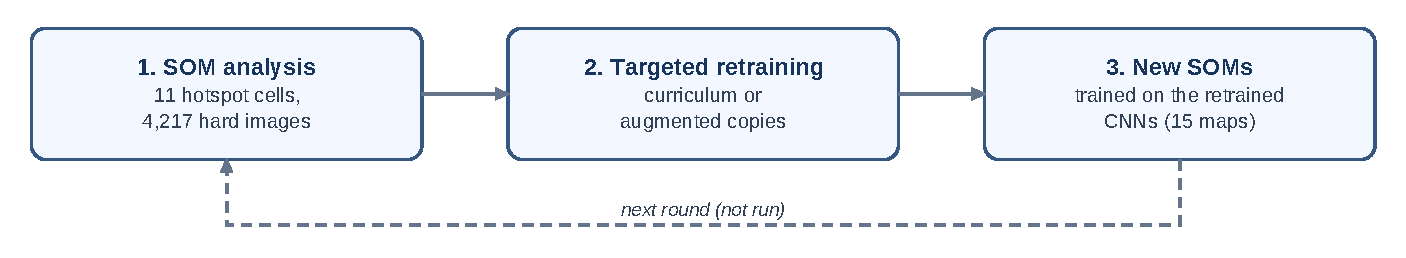
\includegraphics[width=0.9\linewidth]{diagrams/guided_retraining_loop.pdf}
\caption{The feedback loop of Phase 4. The dashed arrow marks a next round, which we did not run.}
\label{fig:loop}
\end{figure}

After retraining, we pull the 84 numbers out of each retrained CNN again and train a new 15$\times$15 SOM on them (the standard, SOM-guided augmentation and random augmentation arms, 5 seeds each). We measure these new maps on the validation images only: purity, the share of impure cells, the topological error, and the error rate in each map's 11 worst cells.
The five statements about the maps (more pure cells, fewer errors in the hotspots, each against the standard arm and the random control, and no loss of map order) were fixed before this run.

\subsection{End-to-end comparison}

Two paths are compared on the same test images (Figure~\ref{fig:endtoend}). In path~1 (CF1), an image goes through the CNN and gets a prediction.
In path~2 (CF2), the CNN has first been retrained with the help of the SOM (SOM-guided augmentation, Phase 4), and the image then goes through this retrained CNN. Each path gives a confusion matrix, CF1 and CF2 (Figure~\ref{fig:cf}). The comparison shows how SOM-guided retraining changes the predictions.
For a fair comparison, CF1 is not the single Phase 1 model but the average over the five seeds of the \emph{standard} retraining arm (99.11\% test accuracy, against 99.18\% for the single Phase 1 model). Both arms use the same recipe, data and seeds, so any difference comes from the SOM guidance.

\begin{figure}[H]
\centering
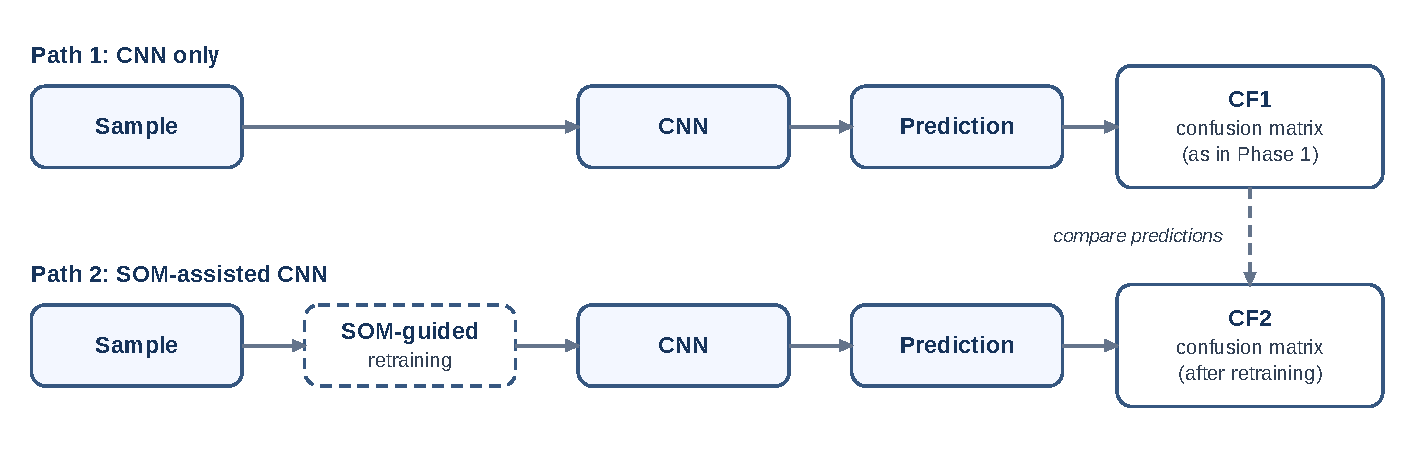
\includegraphics[width=0.9\linewidth]{diagrams/end_to_end_comparison.pdf}
\caption{End-to-end comparison: sample $\rightarrow$ CNN $\rightarrow$ prediction (CF1) against sample $\rightarrow$ SOM-guided retraining $\rightarrow$ CNN $\rightarrow$ prediction (CF2), on the same test samples. The dashed box is the step that uses the SOM.}
\label{fig:endtoend}
\end{figure}

\section{Results}
\label{sec:results}

\subsection{Leakage control}

All development choices use the training and validation images only. The scaler, the SOM, k-means and the nearest-neighbor reference set are fitted on training embeddings. All error statistics are computed on validation images.
The test images were used once, to score the baseline CNN, and the SOM analysis does not use them. The evaluation rules (grid comparison, hotspot rule, number of splits and shuffles, seeds) were set before the results were looked at.
One caution: we chose the CNN checkpoint using the validation images, so these images are not completely untouched by model development.
In Phase 3 the CNN and SOM stay frozen, the alarm threshold comes from the training images, the MNIST test split is not used, and the SVHN images are used only for scoring, never for fitting or choosing a setting. Because the SVHN results were seen before the extra comparisons were run, those comparisons are labelled exploratory. The held-out-digit test was fixed before it was run; its unknown digits are never used for training, choosing an epoch, fitting or setting a threshold.
In Phase 4 the hard pools, the altered copies and the training use training images only. The 11 hotspots were chosen from validation errors, which is why the final judgement uses the test split. The success criteria and thresholds were written down and stamped before the test split was opened, and it was opened once. The new SOMs in the re-analysis are measured on validation images only.

\subsection{Phase 1: Baseline CNN}

The LeNet-5 gets 99.18\% of the test images right (10,414 of 10,500; 95\% Wilson interval 98.99--99.34\%), with a macro F1-score of 0.9918. It makes 92 mistakes on the validation images
(its average confidence is 0.997 when it is right and 0.833 when it is wrong) and 29 on the 49,000 training images. The most common validation confusions are $5\rightarrow0$, $9\rightarrow4$ and $4\rightarrow9$ (six each).

\subsection{Phase 2: SOM structure and where mistakes gather}

On the validation images the 15$\times$15 map has a QE of 1.041 (training: 1.039) and a TE1 of 6.18\%. Its cells follow the digit classes: the purity is 98.19\% on validation images, against 17.4\% (95\% range 17.0--17.7\%) with shuffled labels ($p=0.001$).

The CNN's mistakes gather in a few hotspot cells (Figure~\ref{fig:maps} and Table~\ref{tab:phase2}). The 11 hotspot cells of the 15$\times$15 map hold 11.1 times their fair share of the mistakes (95\% range 6.1--17.6), against about 1 by chance ($p=0.005$).
The result is similar on the 10$\times$10 and 20$\times$20 maps. The error rate of a cell goes down as its purity goes up, and goes up as its digit mix grows, far beyond chance on all three grids.
The three most frequent confusions (4 called 9, 5 called 0 and 9 called 4) each fall on only four or five cells, mostly among the cells of the digit they were mistaken for. The pictures of the mistakes in the hotspot cells suggest that many involve digits that share strokes (4 and 9, 7 and 9, 5, 6 and 8) and that some are unusual handwriting.
A finer grid does not predict mistakes better (the AUROC difference between 20$\times$20 and 15$\times$15 is $+0.001$, range $-0.100$ to $+0.089$), but with only 92 mistakes we cannot detect differences smaller than about 0.1 AUROC.

\begin{table}[H]
\centering
\renewcommand{\arraystretch}{1.12}
\small
\begin{tabular}{|l|c|c|c|}
\hline
\textbf{Measure (validation images)} & \textbf{10$\times$10} & \textbf{15$\times$15} & \textbf{20$\times$20} \\ \hline
Hotspot cells & 5 & 11 & 20 \\ \hline
Concentration ratio (95\% range) & 10.5 (5.4--17.3) & 11.1 (6.1--17.6) & 13.4 (8.0--19.3) \\ \hline
Chance level (median) & 0.98 & 0.94 & 0.93 \\ \hline
Spearman, error rate vs.\ purity & $-0.755$ & $-0.810$ & $-0.766$ \\ \hline
Spearman, error rate vs.\ digit mix (entropy) & $+0.778$ & $+0.816$ & $+0.768$ \\ \hline
\end{tabular}
\caption{Where mistakes gather, on three grid sizes (92 validation mistakes). All $p=0.005$. The ratios should not be used to compare grids with each other.}
\label{tab:phase2}
\end{table}

\begin{figure}[H]
\centering
\begin{minipage}[c]{0.40\textwidth}\centering
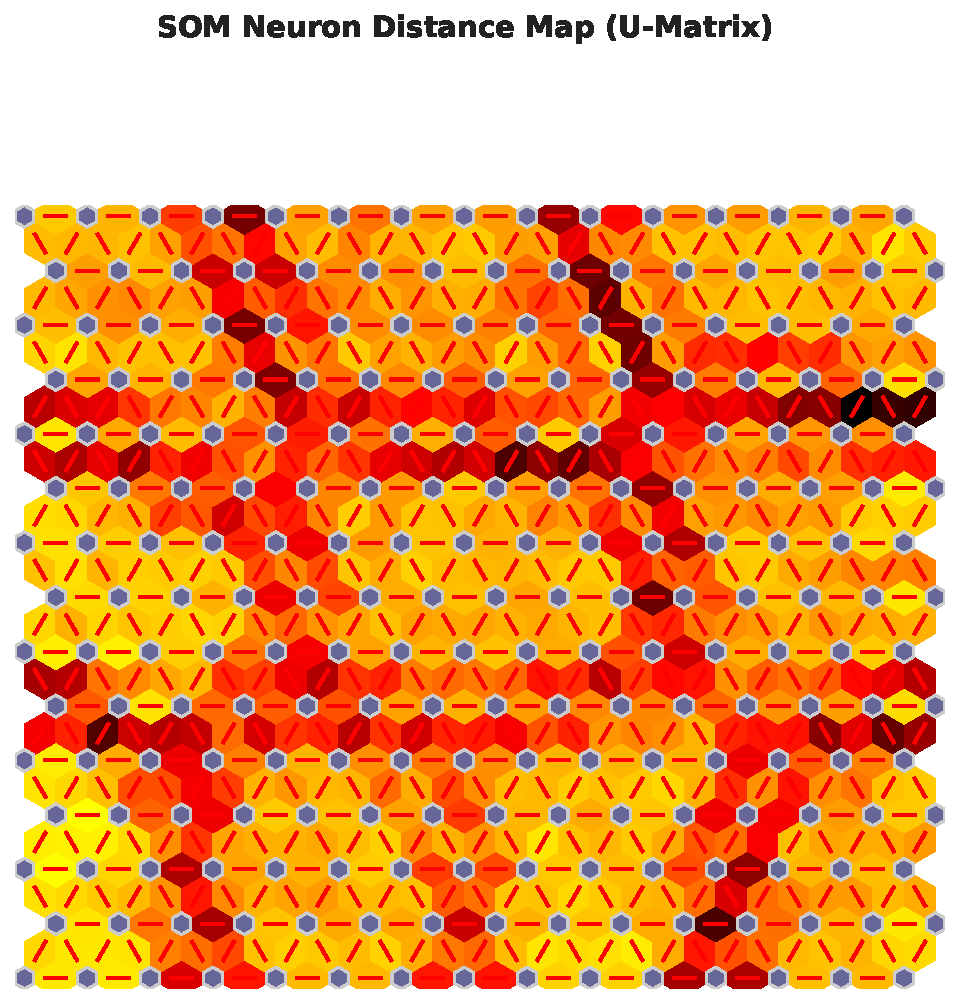
\includegraphics[width=\linewidth,keepaspectratio]{p2_u_matrix.pdf}
\end{minipage}\hfill
\begin{minipage}[c]{0.58\textwidth}\centering
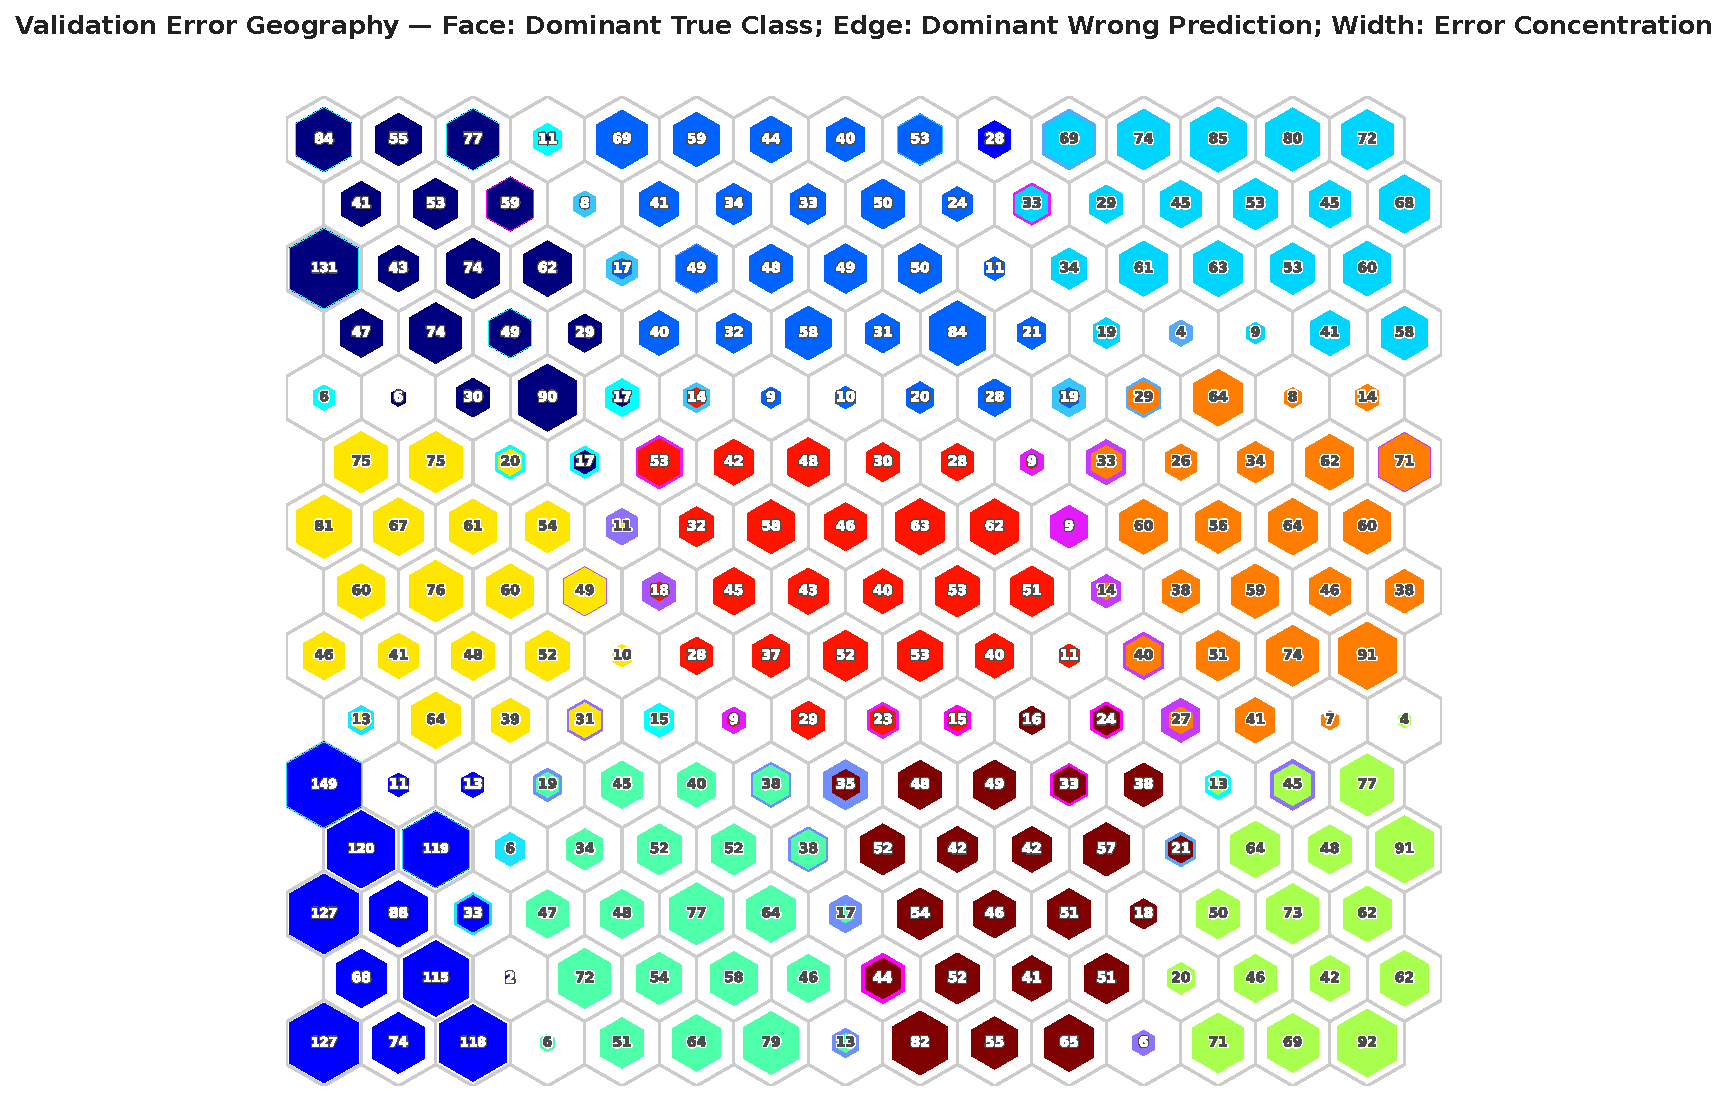
\includegraphics[width=\linewidth,keepaspectratio]{p2_validation_complex_error_map.pdf}
\end{minipage}
\caption{Left: U-matrix of the 15$\times$15 SOM (high values mark borders between groups of cells). Right: validation error map (fill: most common true digit; edge: most common wrong answer; size: how many mistakes).}
\label{fig:maps}
\end{figure}

\subsection{Comparison with baselines}

Table~\ref{tab:error-pattern-baselines} compares the SOM with the baselines on the same validation images. A SOM cell and a k-means cell find mistakes equally well (AUROC 0.685 and 0.693, with overlapping ranges).
Nearest-neighbor impurity does much better (0.874), and the CNN's own confidence does best (0.981). The SOM's hotspots are smaller than those of k-means (1.6\% of the images against 3.8\%), and they catch a similar share of the mistakes (18\% against 20\%).
This is why the SOM has a higher concentration ratio. The hotspot-size numbers are exploratory.
The gap to the per-image scores is large when they get the same budget: flagging the 1.6\% of images with the lowest confidence catches 53.3\% of the mistakes (95\% interval 44.5--64.3\%), and kNN impurity catches 48.7\%, against 18.1\% in the SOM's hotspot cells (exploratory, added after the results were seen).

{\setlength{\tabcolsep}{3pt}\begin{table}[H]
\centering
\renewcommand{\arraystretch}{1.15}
\small
\begin{tabular}{|>{\raggedright\arraybackslash}p{0.25\textwidth}|>{\raggedright\arraybackslash}p{0.19\textwidth}|>{\raggedright\arraybackslash}p{0.10\textwidth}|>{\raggedright\arraybackslash}p{0.14\textwidth}|>{\raggedright\arraybackslash}p{0.10\textwidth}|>{\raggedright\arraybackslash}p{0.10\textwidth}|}
\hline
\textbf{Score} & \textbf{AUROC (95\% range)} & \textbf{Average precision} & \textbf{Hotspot ratio} & \textbf{Images in hotspots} & \textbf{Errors in hotspots} \\ \hline
SOM 15$\times$15 cell error rate & 0.685 (0.624--0.738) & 0.053 & 11.1 (6.1--17.6) & 1.6\% & 18.1\% \\ \hline
k-means, 225 clusters, cell error rate & 0.693 (0.651--0.729) & 0.034 & 5.6 (4.6--6.1) & 3.8\% & 20.4\% \\ \hline
kNN impurity ($k=15$) & 0.874 (0.829--0.917) & 0.228 & n/a & n/a & n/a \\ \hline
CNN max-softmax probability & 0.981 (0.974--0.987) & 0.336 & n/a & n/a & n/a \\ \hline
\end{tabular}
\caption{How well each score finds the 92 validation images that the CNN gets wrong (10,500 images in total). AUROC ranges come from repeated half-splits for the cell scores, and from bootstrap resampling for kNN impurity and max-softmax. Hotspot ratio: share of mistakes divided by share of images in the 11 hotspot cells, chosen on one half and measured on the other. For k-means: median of 10 seeds, with the lowest and highest in brackets. Chance level is about 1 ($p=0.005$ for the SOM and for every k-means seed). n/a: kNN impurity and max-softmax give each image its own score and do not group images into cells, so hotspots are not defined for them.}
\label{tab:error-pattern-baselines}
\end{table}
}

\subsection{Phase 3: Novelty detection}\label{sec:p3results}

Table~\ref{tab:novelty} compares the scores on the same images: 10,500 MNIST validation images as normal data and 26,032 SVHN test images as novel data. The SOM's quantization error separates the two sets well (AUROC 0.981, 95\% interval 0.979--0.983). Shuffling the labels 1,000 times gives a mean AUROC of 0.500, and a random score gives 0.505, so the separation is far from chance.
At the fixed threshold the alarm fires on 96.2\% of the SVHN images and on 5.1\% of the MNIST validation images.

But two simpler scores do better. Energy (0.9998) and the maximum softmax probability (0.9985) rank the novel images higher than QE does. The paired difference between QE and max-softmax is $-0.017$ AUROC (95\% interval $-0.019$ to $-0.015$), so for these fixed images the confidence score is clearly better.
The nearest-neighbor distance (0.977) is close to QE, so the grid itself adds little over plain closeness to the training embeddings. Mahalanobis is weaker (0.776), and the SOM's U-matrix score (0.970) is slightly below QE.

Two scores fall \emph{below} 0.5, which means they rate SVHN images as more normal than MNIST images: Isolation Forest (0.238) and the autoencoder (0.008). The cause is that SVHN embeddings are much shorter than MNIST ones (average length 5.8 against 40.3), and short embeddings are easy to rebuild.
With standardized inputs the autoencoder rises to AUROC $0.979 \pm 0.017$ over five seeds. We keep the original numbers and did not flip any score after seeing the SVHN labels. The same length effect may explain part of QE's own result. QE and embedding length have a Spearman correlation of $-0.83$, and on the small set of images with MNIST-like lengths (only 8 SVHN images) QE's AUROC is 0.72 (95\% interval 0.58--0.84), which is very uncertain.

The SOM's own contribution is where the novel images land (Figure~\ref{fig:overlay}). All 26,032 SVHN images fall on only 28 of the 225 cells, and a single cell (cell 79, mostly 4s) receives 86.5\% of them. The 996 images missed at the threshold fall in 23 cells, 355 of them in the same cell 79.

\begin{table}[H]
\centering
\renewcommand{\arraystretch}{1.12}
\small
\begin{tabular}{|l|c|c|c|}
\hline
\textbf{Novelty score} & \textbf{AUROC} & \textbf{AUPR} & \textbf{FPR at 95\% TPR} \\ \hline
Energy & 0.9998 & 0.9999 & 0.0004 \\ \hline
Maximum softmax probability & 0.9985 & 0.9994 & 0.0078 \\ \hline
SOM quantization error$^\dagger$ & 0.9811 & 0.9766 & 0.0453 \\ \hline
Nearest-neighbor distance ($k=5$) & 0.9766 & 0.9739 & 0.0592 \\ \hline
SOM U-matrix score$^\dagger$ & 0.9696 & 0.9865 & 0.0701 \\ \hline
One-Class SVM$^\dagger$ & 0.9604 & 0.9764 & 0.1794 \\ \hline
Mahalanobis distance & 0.7764 & 0.7859 & 0.3131 \\ \hline
Isolation Forest$^\dagger$ & 0.2383 & 0.5552 & 0.8718 \\ \hline
Autoencoder (unscaled inputs)$^\dagger$ & 0.0077 & 0.4979 & 0.9999 \\ \hline
\end{tabular}
\caption{Novelty detection with 10,500 MNIST validation images as normal data and 26,032 SVHN test images as novel data. Rows marked $^\dagger$ come from the original benchmark (one recorded seed); the others come from a later run on the same images. A random score gives AUROC 0.505. FPR at 95\% TPR is a proportion. The CNN and SOM are fixed, so the intervals (QE: 0.979--0.983; energy: 0.9997--0.9999) show sampling uncertainty only, not variation between trainings. For that variation: on the 15 CNNs retrained in Phase 4 (each with its own new SOM), QE's AUROC on the same images ranged from 0.965 to 0.993 (Section~\ref{sec:p4results}). These comparisons were set up after the SVHN results were seen, so they are exploratory.}
\label{tab:novelty}
\end{table}

\begin{figure}[H]
\centering
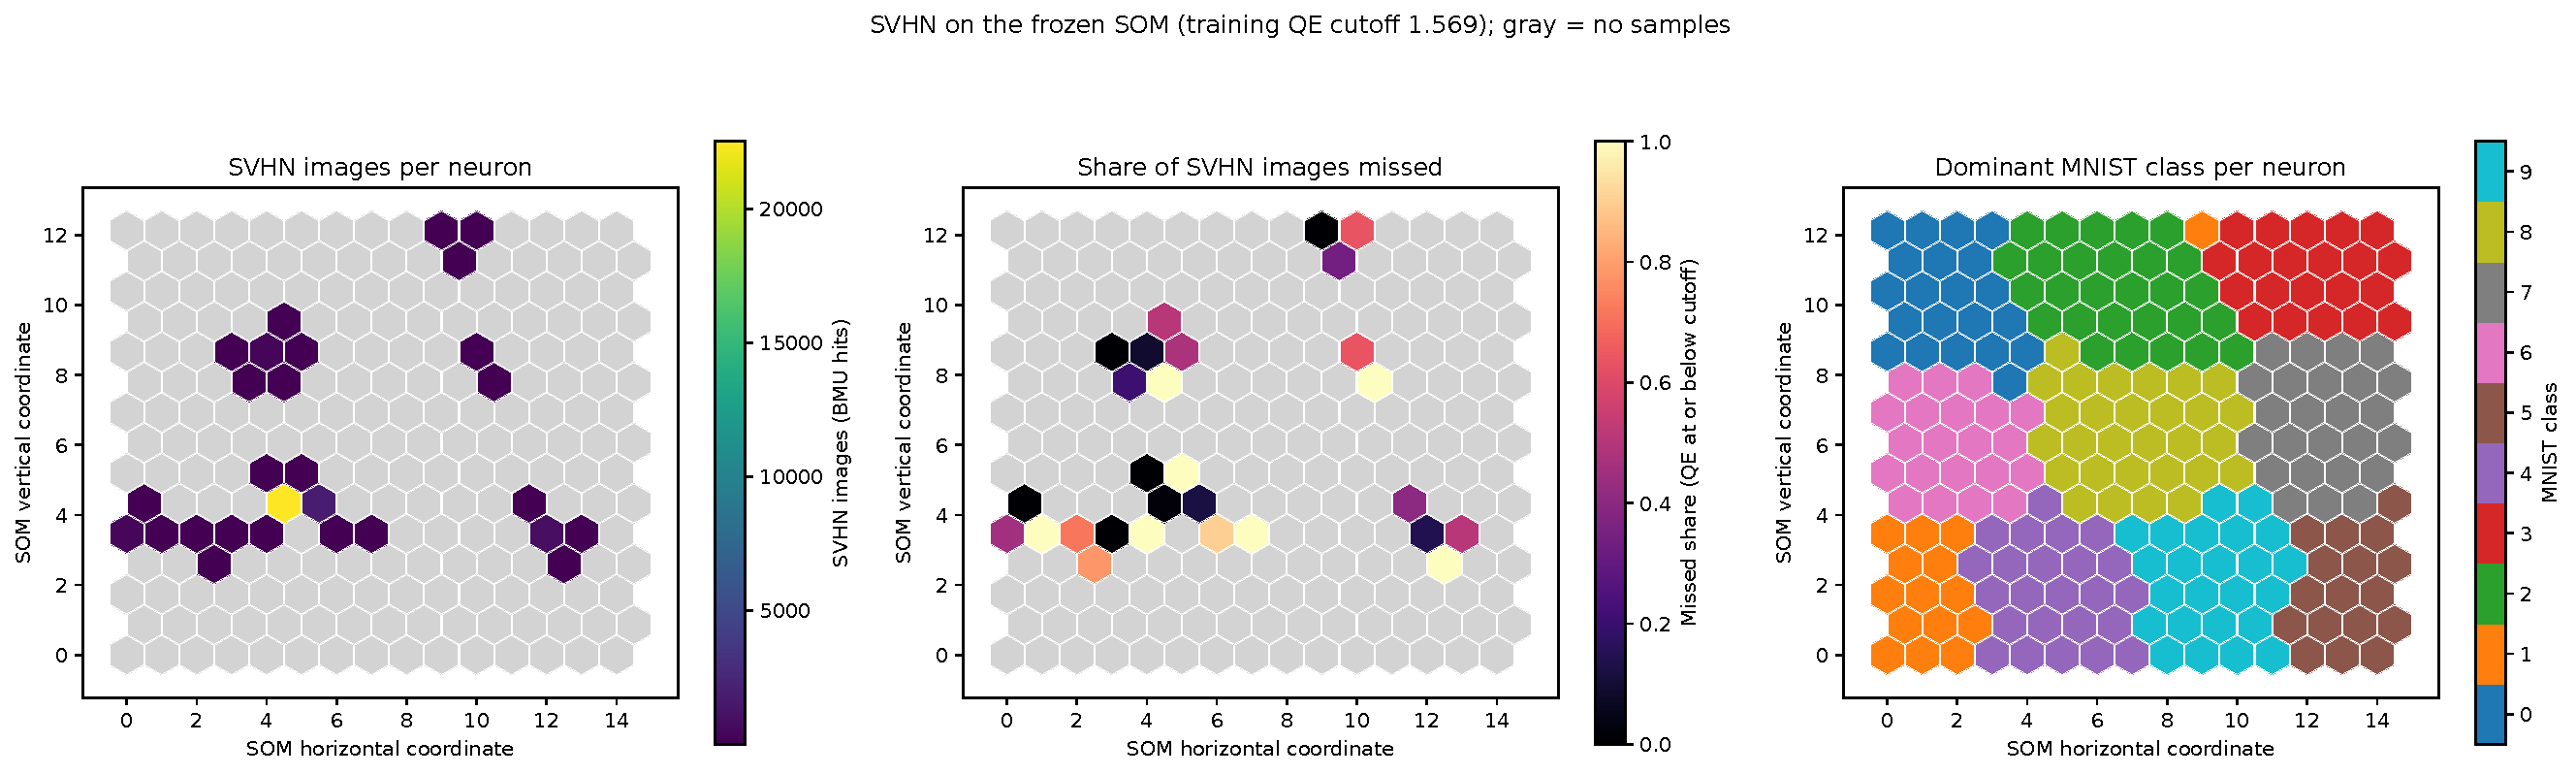
\includegraphics[width=0.95\textwidth,keepaspectratio]{p3_svhn_som_overlay.pdf}
\caption{Where the SVHN test images land on the 15$\times$15 SOM: images per cell (left), the share missed at the threshold, and the most common MNIST digit of each cell. Descriptive only.}
\label{fig:overlay}
\end{figure}

\textbf{Near novelty: held-out digits.} Table~\ref{tab:heldout} gives the results. The networks reach 99.1--99.4\% accuracy on the known digits. The SOM detects digits it has never seen in every split (H1 shown; AUROC 0.860 to 0.957, every interval above 0.5; a label-shuffle control gives 0.500). Here the result is not a length effect: embedding length alone gives only 0.63 to 0.89, and QE and length are weakly related (Spearman $-0.32$ to $+0.01$).
But the SOM is not shown to beat max-softmax: it is lower in 4 of the 5 splits, by 0.032 AUROC on average (95\% interval $-0.095$ to $+0.032$), so H2 is inconclusive. It is also not shown to be within 0.01 of max-softmax, energy or Mahalanobis (H3 inconclusive for all three); the splits vary too much for five values to settle these. Plain nearest-neighbor distance on the same embeddings beats QE in all five splits ($-0.054$, interval $-0.084$ to $-0.024$; H4 shown in the opposite direction): the 225 cells of the map lose detail that the training embeddings keep.
As with SVHN, the map shows where new inputs land: 90\% of the novel images fall in 33 to 55 of the 225 cells, while 90\% of the normal images need 166 to 174.

\begin{table}[H]
\centering
\renewcommand{\arraystretch}{1.12}
\footnotesize
\setlength{\tabcolsep}{4pt}
\begin{tabular}{|c|c|c|c|c|c|c|}
\hline
\textbf{Split} & \textbf{Unknown} & \textbf{SOM QE} & \textbf{Max-} & \textbf{Energy} & \textbf{Maha-} & \textbf{Nearest} \\
 & \textbf{digits} & & \textbf{softmax} & & \textbf{lanobis} & \textbf{neighbor} \\ \hline
1 & 0, 1, 5, 6 & 0.907 & 0.956 & 0.947 & 0.874 & 0.961 \\ \hline
2 & 2, 3, 5, 8 & 0.957 & 0.917 & 0.893 & 0.965 & 0.979 \\ \hline
3 & 1, 5, 6, 7 & 0.860 & 0.958 & 0.959 & 0.916 & 0.948 \\ \hline
4 & 2, 5, 6, 8 & 0.931 & 0.940 & 0.890 & 0.954 & 0.977 \\ \hline
5 & 0, 4, 5, 8 & 0.905 & 0.948 & 0.944 & 0.929 & 0.965 \\ \hline
\multicolumn{2}{|c|}{\textbf{Mean}} & \textbf{0.912} & \textbf{0.944} & \textbf{0.927} & \textbf{0.927} & \textbf{0.966} \\ \hline
\multicolumn{2}{|c|}{QE minus score} & -- & $-0.032$ & $-0.015$ & $-0.015$ & $-0.054$ \\
\multicolumn{2}{|c|}{(95\% interval)} & & ($-0.095$, $+0.032$) & ($-0.097$, $+0.068$) & ($-0.056$, $+0.025$) & ($-0.084$, $-0.024$) \\ \hline
\end{tabular}
\caption{Near novelty: AUROC for detecting the 4 held-out digits (about 4,100 validation images per split) among the 6 known digits (about 6,400), with a new LeNet-5 and a new 15$\times$15 SOM trained on the known digits of each split. Within a split, the bootstrap intervals are about $\pm0.005$ wide. The protocol, splits and statements were fixed before the run; the MNIST test split was not used.}
\label{tab:heldout}
\end{table}

\subsection{Phase 4: Guided retraining}\label{sec:p4results}

Table~\ref{tab:retraining} gives the main results. \textbf{Targeted augmentation helped where the SOM pointed.} The SOM-guided arm cut the error on the 146 test images in the hotspots from 11.4\% to 7.8\%. In numbers of images this is about 17 wrong for normal training and about 11 for the guided arm.
The drop is clear against normal training ($-3.6$ points, 95\% interval $-5.8$ to $-1.4$) and against the same number of random images ($-2.5$ points, interval $-4.5$ to $-0.7$). The error on the other 10,354 images did not rise ($-0.05$ points, interval $-0.13$ to $+0.02$), and overall accuracy went from 99.11\% to 99.21\%, about 11 fewer mistakes out of 10,500. This is a small gain: MNIST is already 99\% correct, and the gain varies between seeds.

\textbf{But the SOM was not a better picker than confidence.} Choosing the images with the lowest maximum softmax probability gave almost the same result (99.25\%, 8.5\% in the hotspots). The difference to the SOM-guided arm is $-0.7$ points (interval $-2.9$ to $+1.2$), so we cannot tell them apart. Adding the copies gradually instead of all at once was worse (hotspot error 11.2\%, $+3.4$ points).

\textbf{Curriculum learning did not help.} The curriculum CNNs were clearly worse than normal training (98.66\% and 98.69\% against 99.11\%, about 47 more mistakes out of 10,500). They were behind from the first epochs and never caught up. We did not test why; one possible reason is that they only ever see 40\% of the hard images.
Forgetting was not a problem: in every arm the largest drop in validation accuracy from one epoch to the next was about 0.6 points or less, and for the SOM-guided augmentation the error outside the hotspots stayed at the normal level.

\begin{table}[H]
\centering
\renewcommand{\arraystretch}{1.12}
\small
\begin{tabular}{|>{\raggedright\arraybackslash}p{0.31\textwidth}|C{0.14\textwidth}|C{0.14\textwidth}|C{0.15\textwidth}|C{0.13\textwidth}|}
\hline
 & \multicolumn{2}{c|}{\textbf{Test images}} & \multicolumn{2}{c|}{\textbf{New SOM (validation)}} \\ \hline
\textbf{Selection of hard images} & \textbf{Accuracy (\%)} & \textbf{Hotspot error (\%)} & \textbf{Hotspot error rate} & \textbf{Purity} \\ \hline
None (normal training, CF1) & 99.11 & 11.4 & 0.229 & 0.982 \\ \hline
Random (augmentation) & 99.18 & 10.3 & 0.206 & 0.981 \\ \hline
Least confident (augmentation) & 99.25 & 8.5 & 0.193$^{\dagger}$ & 0.983$^{\dagger}$ \\ \hline
SOM-guided (augmentation, CF2) & 99.21 & 7.8 & 0.175 & 0.982 \\ \hline
SOM-guided (curriculum) & 98.66 & 21.4 & n/a & n/a \\ \hline
\end{tabular}
\caption{Retraining results, mean over 5 seeds. Test columns: accuracy on all 10,500 test images and error on the 146 test images in the hotspots. New SOM columns: error rate in the 11 worst cells and purity of a new 15$\times$15 SOM trained on each retrained CNN, measured on validation images (the hotspots are chosen again for each map). The Phase 1 model (99.18\%) is a single run and is not in this table. n/a: not re-analysed. The SOM re-analysis protocol fixed in advance to re-analyse only normal training and the two augmentation arms with a measured effect (SOM-guided and random). $^{\dagger}$The least-confident arm was re-analysed later, in a secondary run added after these results were seen; the curriculum arm was not re-analysed. Novelty detection after retraining is reported in the text below.}
\label{tab:retraining}
\end{table}

\textbf{What the new maps show.} The hotspots of the new SOM after SOM-guided augmentation hold fewer mistakes than after normal training (error rate 0.175 against 0.229, lower in all 5 seeds). But the cells are not purer (0.982 for both), so the class boundaries did not get sharper by our measure. Against random augmentation the hotspot drop (0.175 against 0.206) is not clear, since its interval includes zero. In a secondary run, added after these results were seen, we re-analysed the least-confident arm in the same way. Its new maps have a hotspot error rate of 0.193, which is not clearly below normal training ($-0.036$, interval $-0.093$ to $+0.021$), and SOM guidance is not clearly better than it, either on hotspot error ($-0.018$, $-0.076$ to $+0.039$) or on purity. So with five seeds we cannot show that SOM guidance shrinks the weak regions of the new map more than choosing the least-confident images.
The map stayed as well ordered as before (topographic error did not rise). Figure~\ref{fig:reanalysis} shows the measures for each seed. So the map after retraining has smaller weak regions, but it does not have cleaner classes.

\textbf{Novelty detection after retraining.} We repeated the Phase 3 test (MNIST validation images against SVHN) on every retrained CNN, with a new SOM for each one and the same four detectors as before. The SOM still separates SVHN from MNIST in every retrained network (lowest AUROC 0.965). SOM-guided retraining raised its AUROC slightly on average (0.984 against 0.976 for normal training), but the difference is not clear ($+0.008$, 95\% interval $-0.014$ to $+0.030$), and the same holds against random augmentation ($+0.0005$, $-0.016$ to $+0.017$). Max-softmax (about 0.998) and energy (about 0.9996) stay better in every network. Embedding length alone still separates SVHN almost perfectly (0.9998 to 0.9999), so, as in Phase 3, the SVHN result says more about SVHN's short embeddings than about the map.

\begin{figure}[H]
\centering
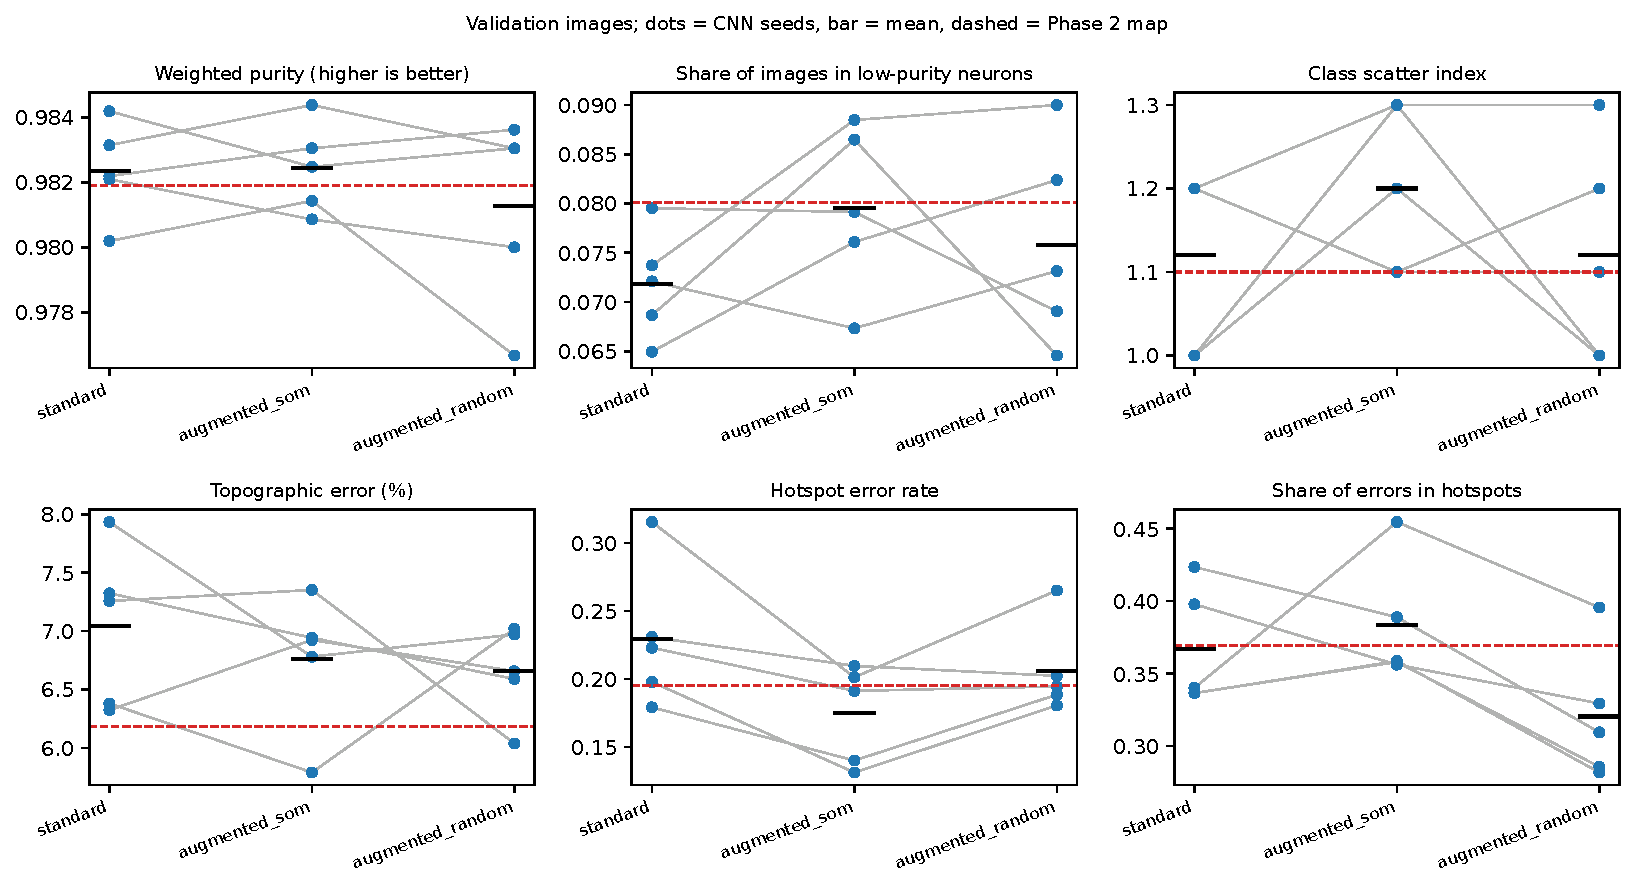
\includegraphics[width=\textwidth]{p4_map_measures_by_arm.pdf}
\caption{Measures of the new SOMs on validation images. Each dot is one CNN seed, the black bar is the mean over seeds, and the red dashed line is the Phase 2 map.}
\label{fig:reanalysis}
\end{figure}

\subsection{End-to-end comparison}

Figure~\ref{fig:cf} shows CF1 (normal training), CF2 (SOM-guided augmentation) and their difference on the same 10,500 test images, averaged over 5 seeds. The diagonal is the correct answers. Most of the change is a small set of confusions that become a little less frequent (blue) or a little more frequent (red).
Net, CF2 has about 11 fewer mistakes than CF1 (82.6 against 93.2 on average), of which about 5 fewer are on the 146 hotspot images. Individual mistakes move a lot, however: for each seed the SOM-guided CNN fixes about 40 of the standard CNN's mistakes and makes about 30 new ones, and the net gain over all images ranges from $-12$ to $+31$ between seeds.
The gain on the hotspot images is more stable (1 to 8 fewer mistakes in every seed). We therefore read the end-to-end gain as small and not reliable on its own, and the hotspot gain as the clearer effect.

\begin{figure}[H]
\centering
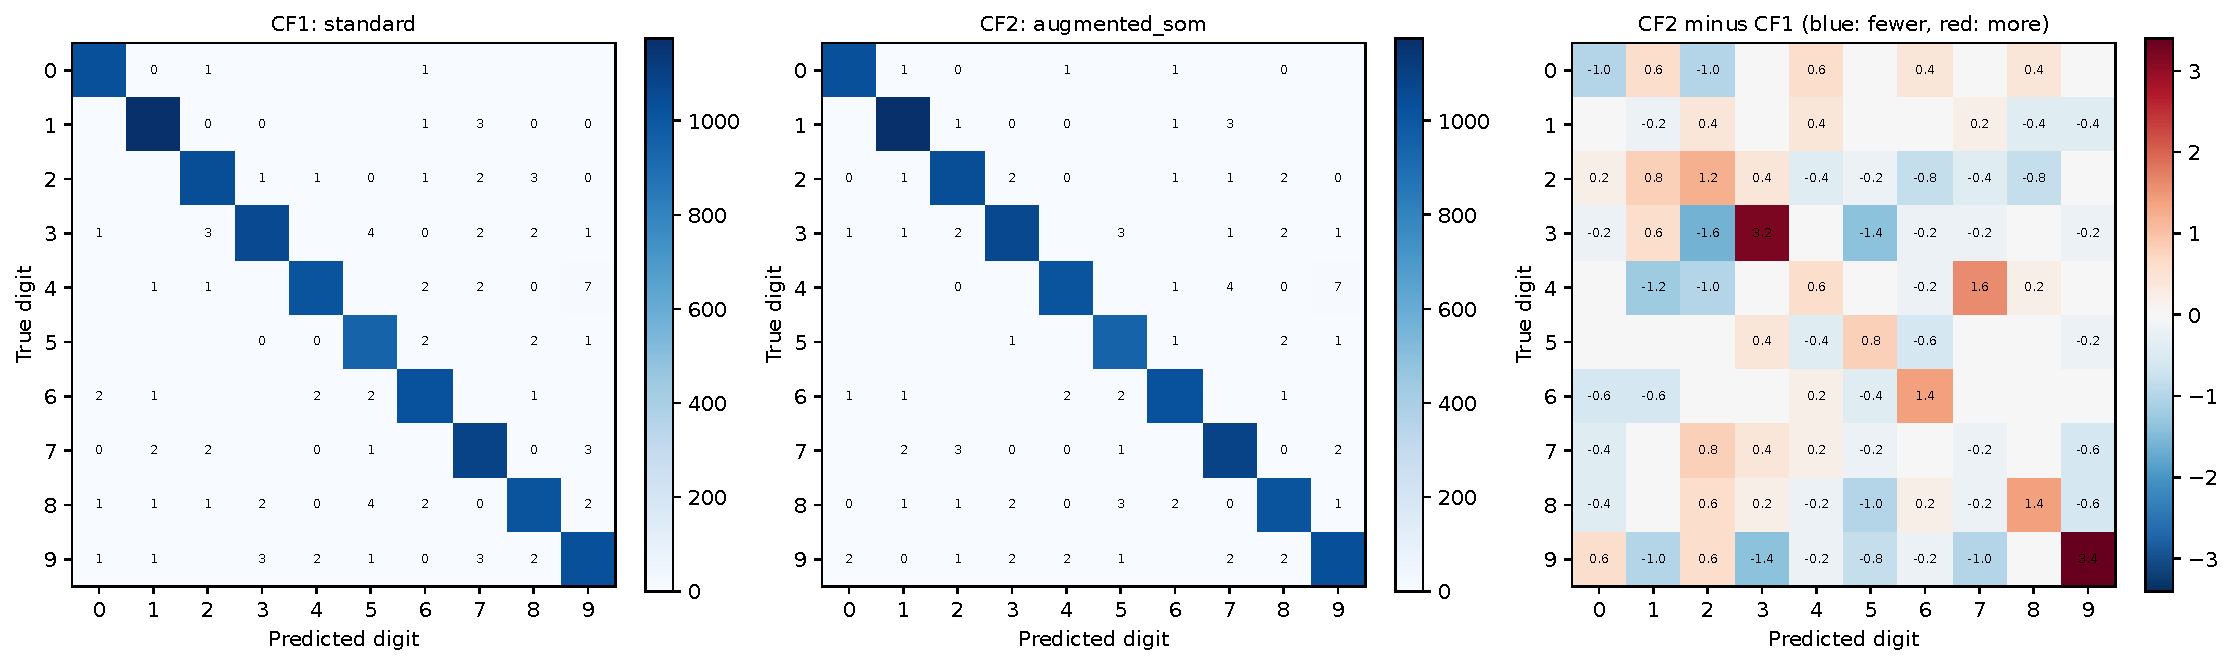
\includegraphics[width=\textwidth]{p4_confusion_standard_vs_augmented_som.pdf}
\caption{CF1 (normal training) and CF2 (SOM-guided augmentation): mean test confusion matrices over 5 seeds, and their difference (blue: fewer cases, red: more).}
\label{fig:cf}
\end{figure}

\section{Discussion and Limitations}

On MNIST the SOM turns the 84 numbers of each embedding into a map where the digit classes form clean regions and the mistakes sit in the few cells where digits mix. This holds on three grid sizes and against chance.
But if the only goal were to find likely mistakes, the maximum softmax probability would be the better tool. So the value of the SOM lies in the picture it gives, and possibly in novelty detection and retraining.
Mistakes are also farther from their cell than correct images are (average distance 1.349 against 0.960), which may help find unfamiliar inputs.

This held up in Phase 3: the SOM's quantization error separates SVHN from MNIST well (AUROC 0.981), but energy and max-softmax separate them better, and part of the SOM's result may come from the short SVHN embeddings. On held-out digits, where length is not the explanation and max-softmax is far from perfect, the SOM still did not win: it was not shown to beat max-softmax, and plain nearest-neighbor distance beat it in every split. So even the setting in which a map-based detector was expected to have its best chance does not favor it on MNIST. As in Phase 2, the CNN's own confidence is the stronger signal, and the SOM adds a view of where the novel images and the missed ones land.
In Phase 4 the SOM's hotspots were a useful guide for retraining: augmenting the hard images from those cells lowered the mistakes there without hurting the rest, and the new map has smaller weak regions. But picking the least confident images gave about the same gain, so the SOM is a good \emph{explainer} of where to look, not a better \emph{selector}.
Letting the hard images in slowly (curriculum) did not help, and the cells of the new map did not become purer. The whole loop (analyze, retrain, analyze again) works, but the gains on MNIST are small because the CNN is already 99\% correct.

\textbf{Limitations.}
(1)~We have only 92 validation mistakes, so the intervals are wide, and differences below about 0.1 AUROC cannot be seen.
(2)~MNIST is easy. A harder dataset (Fashion-MNIST) is needed before we can draw general conclusions.
(3)~The grid comparison could not separate the three grid sizes, so the choice of 15$\times$15 rests on a trade-off between purity and topological error, not on a clear winner.
(4)~The baseline comparison covers only the 15$\times$15 map and uses three k-means starts per seed.
(5)~We also used the validation images to choose the CNN checkpoint.
(6)~The SVHN results use one CNN and one SOM, so their intervals show only sampling noise, and the SVHN comparisons were set up after the SVHN results were seen. The held-out-digit test uses five class splits with one network and one SOM each; the splits share images and digits, so its t-intervals may be too narrow, and the random draw left the digits unbalanced (5 is unknown in four splits, 9 in none).
(7)~In Phase 4 only 146 test images lie in the hotspots, so the hotspot intervals are wide. The hotspots come from the SOM, which gives the SOM-guided arms a built-in advantage on hotspot error. The pools come from one SOM, and five seeds can only separate fairly large differences.
(8)~The first set of augmentation settings (shifts of up to 2 pixels) failed a check made before training: the validation accuracy of the CNN fell from 99.12\% to 95.83\% on the altered images. We lowered the shift to 1 pixel, which passed (98.21\%), and all augmentation results use this version.
(9)~After retraining, the novelty test again uses only SVHN, whose short embeddings make it easy to detect, and five seeds cannot separate AUROC differences of about 0.01.

\section{Conclusion}

On MNIST, a SOM trained on a CNN's embeddings shows where the CNN's few mistakes gather: in a small set of cells where digits overlap, far beyond chance. The map does not find mistakes or novel inputs better than simple scores, and the CNN's own confidence and energy score do better at both jobs (mistakes: 0.981 against 0.685 AUROC; SVHN: 0.9985 and 0.9998 against 0.981).
Its value is that it shows where. SVHN collapses onto 28 of 225 cells, and the hotspot cells could be used to pick images for retraining. Augmenting the hard images from the hotspots lowered the mistakes there from 11.4\% to 7.8\% without hurting the rest, and the new SOM has smaller weak regions. Curriculum learning did not help, and the cells of the new map did not become purer.
After retraining the SOM still detects SVHN, but no better than before. On held-out digits it detects new classes too, but plain nearest-neighbor distance does better and it is not shown to beat max-softmax. The next step is to repeat the whole study on Fashion-MNIST, where the CNN makes more mistakes and the gains may be larger.

\clearpage
\printbibliography[title={References}]

\end{document}
